\section{The Algorithm -- Theoretical Part} \label{algorithm-theory}

\subsection{A tree of boxes, neighbors and interaction lists}

In order to understand the concepts that will be used to define the algorithm, we need to elaborate more on what we already introduced in the previous section.
As we aim to achieve linear complexity when we evaluate the potentials of the gravitational force, the \gls{fmm} splits the computational domain into a tree of boxes, called quad-tree.
First, divide the square $\Omega$ into $4^L$ equisized smaller boxes, where $L$ is a large enough integer such that each box can only carry a small number of particles.
The leaf boxes of the tree are made up of these $4^L$ equisized small boxes.
Levels, which are the set of all boxes with the same size, are labeled using integers $l = 0, 1, \dots, L$, where $l=0$ is the root.
The root is the original box that contains all the particles.

Given a box $\tau$ \cite{Martinsson2015}:
\begin{itemize}
  \item The parent of $\tau$ is the box on the following higher level that contains $\tau$.
  \item The children of $\tau$ compose the set $L_{\tau}^\text{child}$ of boxes with $\tau$ as their parent.
  \item The neighbors of $\tau$ compose the set $L_{\tau}^\text{nei}$ of boxes that directly touch $\tau$.
  \item The interaction list of $\tau$ is the set $L_{\tau}^\text{int}$ of all boxes $\sigma$ such that $\sigma$ and $\tau$ are on the same level, and do not touch each other, but their parents touch each other.
\end{itemize}

\subsection{A multi-level method}

We have all the tools required to describe the classical \gls{fmm} in $\mathbb{R}^2$ in details.
First, we need to find a minimal square $\Omega$ that holds all the points.
The ideal number of points to have in a box depends on a variety of factors but having 100 points for each box is usually a good starting point \cite{Martinsson2015}.
Next, we split $\Omega$ into smaller boxes as described in the section above, and fix $P$ that determines the accuracy.
The larger $P$, the higher the accuracy, but also higher cost.
The algorithm is as follows \cite{Martinsson2015}:

\begin{enumerate}
  \item Construct the tree and all interaction lists
  \item Compute: $\hat{\vct{q}}^{\tau}=\vct{T}_{\tau}^{\mathrm{ofs}} \vct{q}\left(I_{\tau}\right)$

  For each leaf, replace the original sources by the corresponding outgoing expansions, which are shown as green dots in the \cref{fig:step2}.
  You can compute the outgoing expansions directly from the sources in the box via the outgoing-from-source translation operator.
  This operator results from truncating the outgoing expansion of $\Omega$ to order $P$, which is the vector $\hat{q} \in \mathbb{C}^{P+1}$ with numbers \cite{Martinsson2015}:
  \begin{equation}
    \begin{split}
      \hat{\vct{q}}_0 &= \sum_j^P m_j \\
      \hat{\vct{q}}_k &= - \sum_j^P \frac{m_j}{k} (\vct y - \vct c_\sigma)^k
    \end{split}
  \end{equation}
  \begin{figure}
    \centering
    \subfloat{
      \resizebox{4cm}{4cm}{%
        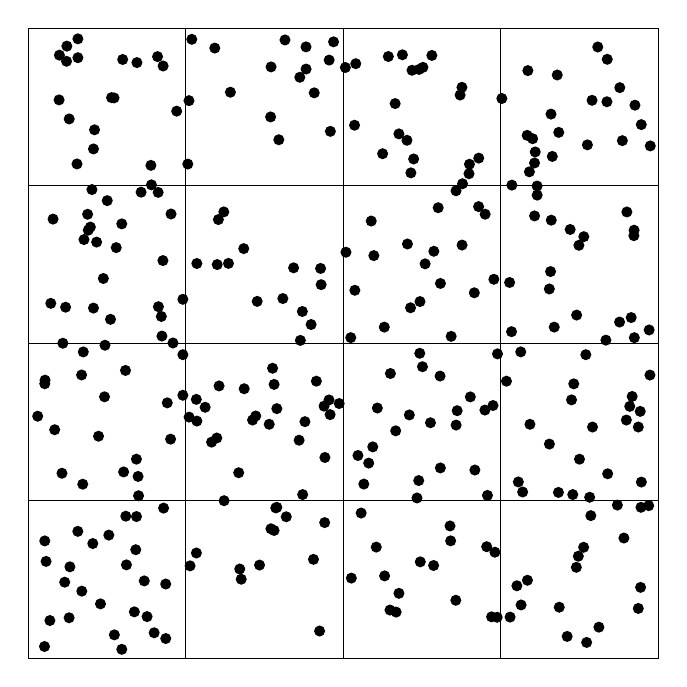
\begin{tikzpicture}
          \pgfmathsetseed{42}
          \draw (0,0) rectangle (8,8);
          \draw[step=2] (0,0) grid (8,8);
          \foreach \x in {1,...,320} {
            \fill (rnd*7.8+0.1, rnd*7.8+0.1) circle (2pt);
          }
        \end{tikzpicture}
      }
    }\hspace{1em}\subfloat{
    \resizebox{4cm}{4cm}{%
      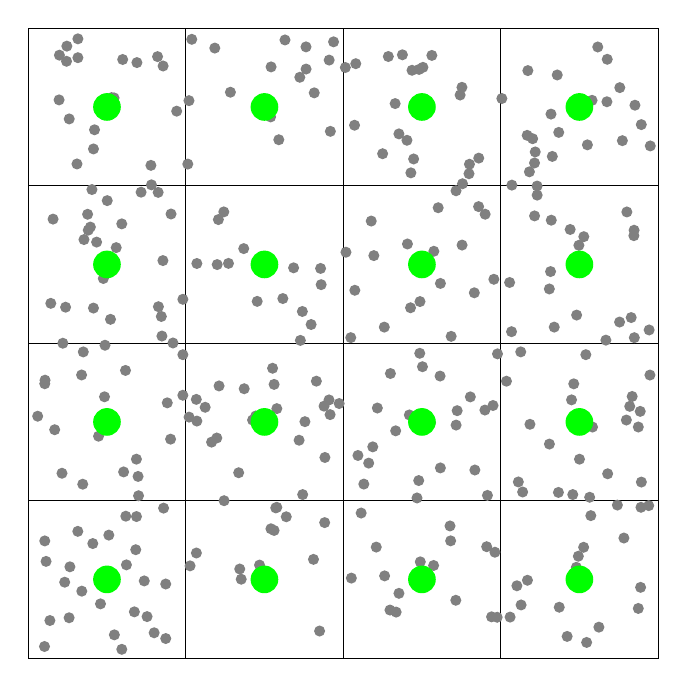
\begin{tikzpicture}
        \pgfmathsetseed{42}
        \draw (0,0) rectangle (8,8);
        \draw[step=2] (0,0) grid (8,8);
        \foreach \x in {1,...,320} {
          \fill[gray] (rnd*7.8+0.1, rnd*7.8+0.1) circle (2pt);
        }
        \foreach \x in {1,3,5,7} {
          \foreach \y in {1,3,5,7} {
            \fill[color=green] (\x, \y) circle (5pt);
        }}
      \end{tikzpicture}
      }
    }
    \caption{Step 2 of \gls{fmm}}
    \label{fig:step2}
  \end{figure}

  \item Compute: $\hat{\vct{q}}^{\tau}=\sum_{\sigma \in \mathcal{L}_{\tau}^{\text {child }}} \vct T_{\tau, \sigma}^{\text {ofo }} \hat{\vct{q}}^{\sigma}$

    In the \nth{3} step, here we look at a box in the next level up.
    For a box $\tau$ that has children, the outgoing expansion is computed not directly from the sources located in the box, but from the outgoing expansions of its children, which are already available.
    We do this by taking the outgoing expansion of its children (shown as green poles in \cref{fig:step3:childs}).
    This way we get the outgoing expanison shown in \cref{fig:step3:last}.
    And this is an expansion that allows me to evaluate potentials outside the blue box.
    So basically we want a compact representation of potentials of the particles in the gray area in \cref{fig:step3:parts} that is valid outside the blue box.
    For any point in the yellow highlighted area in \cref{fig:step3:last}, the outgoing expansions highlighted in yellow in \cref{fig:step3:childs} are all valid.
    Therefore, we already have a compact representation of the potential outside of the blue square, and we move these expansions via a outgoing-from-outgoing translation operator.
    The outgoing-from-outgoing translation operator $\vct T_{\tau, \sigma}^\mathrm{ofo}$ can be derived from truncating the series to the first $P$ terms \cite{Martinsson2015}:

    \begin{equation}
      \begin{split}
        \hat{\vct q}_{0}^{\tau} &= \hat{\vct q}_{0}^{\sigma} \\
        \hat{\vct q}_{k}^{\tau}
          &= - \hat{\vct q}_{0}^{\sigma} \frac{1}{k} \left(\vct c_{\sigma}-\vct c_{\tau}\right)^{k}
             + \sum_{j=1}^{k} \hat{\vct q}_{j}^{\sigma} \mat{k-1 \\ j-1} \left(\vct c_{\sigma}-\vct c_{\tau}\right)^{k-j}
      \end{split}
    \end{equation}

  \begin{figure}
    \centering
    \subfloat{
    \label{fig:step3:parts}
    \resizebox{4cm}{4cm}{%
      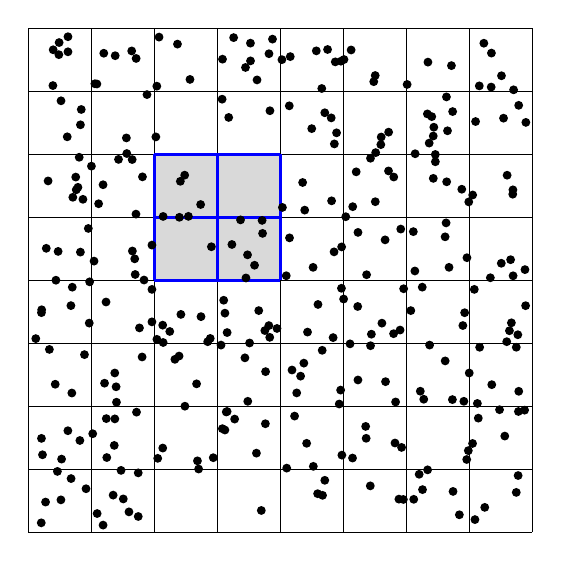
\begin{tikzpicture}[scale=0.8]
        \pgfmathsetseed{42}
        \fill[gray!30] (2,4) rectangle (4,6);
        \draw[step=1] (0,0) grid (8,8);
        \draw[very thick, blue] (2,4) grid (4,6);
        \foreach \x in {1,...,320} {
          \fill (rnd*7.8+0.1, rnd*7.8+0.1) circle (2pt);
        }
      \end{tikzpicture}}
    }\subfloat{%
    \label{fig:step3:childs}
    \resizebox{4cm}{4cm}{%
      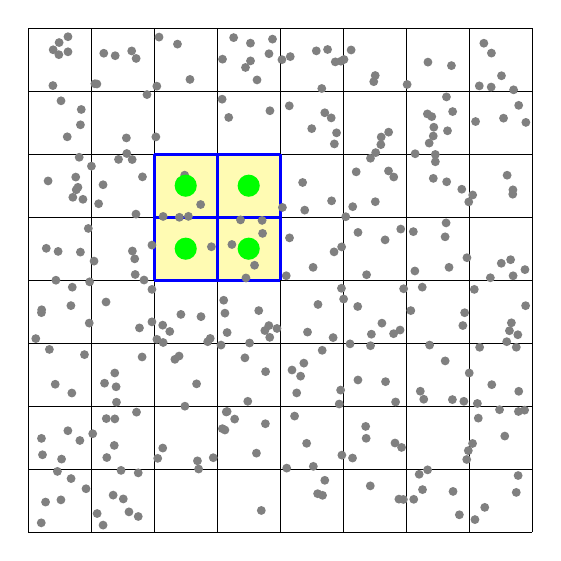
\begin{tikzpicture}[scale=0.8]
        \pgfmathsetseed{42}

        \fill[gray!30] (2,4) rectangle (4,6);
        \fill[yellow!30] (2,4) rectangle (4,6);

        \draw[step=1] (0,0) grid (8,8);
        \draw[very thick, blue] (2,4) grid (4,6);
        \foreach \x in {1,...,320} {
          \fill[gray] (rnd*7.8+0.1, rnd*7.8+0.1) circle (2pt);
        }
        \foreach \x in {2.5,3.5} {
          \foreach \y in {4.5,5.5} {
            \fill[color=green] (\x, \y) circle (5pt);
        }}
      \end{tikzpicture}
      }
    }\subfloat{%
    \label{fig:step3:last}
    \resizebox{4cm}{4cm}{%
      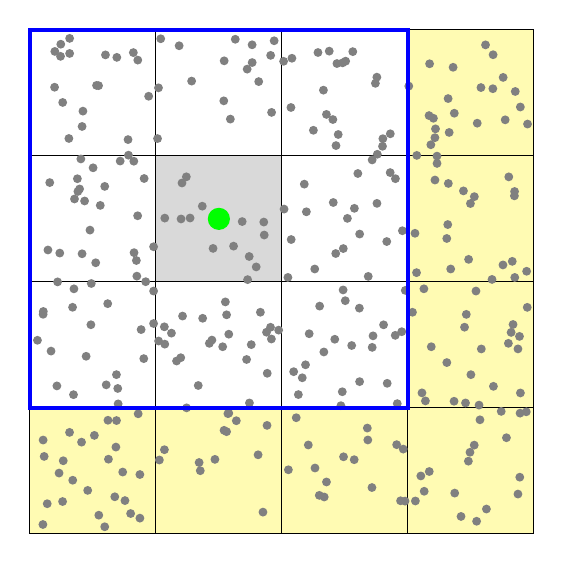
\begin{tikzpicture}[scale=0.8]
        \pgfmathsetseed{42}

        \fill[yellow!30] (0,0) rectangle (8,2);
        \fill[yellow!30] (6,0) rectangle (8,8);

        \fill[gray!30] (2,4) rectangle (4,6);
        \draw[step=2] (0,0) grid (8,8);
        \foreach \x in {1,...,320} {
          \fill[gray] (rnd*7.8+0.1, rnd*7.8+0.1) circle (2pt);
        }
        \fill[color=green] (3,5) circle (5pt);
        \draw[ultra thick, blue] (0,2) rectangle (6,8);
      \end{tikzpicture}
      }
    }
    \caption{Step 3 of \gls{fmm}}
    \label{fig:step3}
  \end{figure}

  \item Compute: $\hat{\vct{u}}^{\tau}=\hat{\vct{u}}^{\tau}+\sum_{\sigma \in \mathcal{L}_{\tau}^{i n t}} \vct T_{\tau, \sigma}^{ifo} \hat{\vct{q}}^{\sigma}$
        and $\hat{\vct{u}}^{\tau}=\hat{\vct{u}}^{\tau}+\vct T_{\tau, \sigma}^{\mathrm{ifi}}
  \hat{\vct{u}}^{\sigma}$

  In the \nth{4} step, we convert outgoing expansions to incoming expansions.
  Loop over all boxes $\tau$, and for each box, collect contributions to its incoming expansion $u^\tau$ from the interaction list.
  In \cref{fig:step4}, the interaction list of the grey highlighted box is shown with the red particles.
  It is the list box for which the grey box needs to collect the incoming expansions.
  This is done by the incoming-from-outgoing translation operator.
  We start at level 2: we want to compute the incoming expansion of the grey highlighted box.
  This is a potential caused by all the red particles in \cref{fig:step4:parts}.
  Also, these boxes are all well-separated, and therefore, we can replace all the red particles by outgoing expansions shown with green dots in \cref{fig:step4:poles}.
  In other words, we add the contributions from all the sources in its interaction list using the incoming-from-outgoing translation operator.
  The incoming-from-outgoing translation operator results from truncating the incoming expansion to the first $P$ terms \cite{Martinsson2015}:
    \begin{equation}
      \begin{split}
        \hat{\vct{u}}_0 &= \hat{\vct{q}}_0 \log(\vct c_\tau - \vct c_\sigma) + \sum_{j=1}^\infty \hat{\vct{q}}_j (-1)^j \frac 1 {(\vct c_\sigma - \vct c_\tau)^j} \\
        \hat{\vct{u}}_k &= -\hat{\vct{q}}_0 \frac 1 {k(\vct c_\sigma - \vct c_\tau)^k} + \sum_{j=1}^\infty \hat{\vct{q}}_j (-1)^j \mat{k+j-1\\j-1} \frac 1 {(\vct c_\sigma - \vct c_\tau)^{k+j}} \\
      \end{split}
    \end{equation}


  \begin{figure}
    \centering
    \subfloat{
    \label{fig:step4:parts}
    \resizebox{4cm}{4cm}{%
      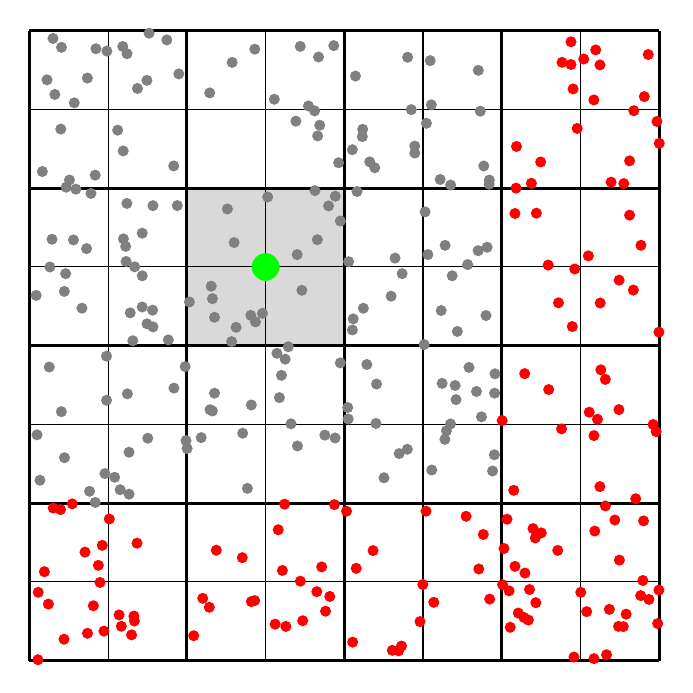
\begin{tikzpicture}
        \pgfmathsetseed{42}

        \fill[gray!30] (2,4) rectangle (4,6);

        \draw[step=1            ] (0,0) grid (8,8);
        \draw[step=2, very thick] (0,0) grid (8,8);

        \foreach \x in {1,...,180} {
          \fill[gray] (rnd*6, rnd*6+2) circle (2pt);
        }
        \foreach \x in {1,...,80} {
          \fill[red] (rnd*8, rnd*2) circle (2pt);
        }
        \foreach \x in {1,...,60} {
          \fill[red] (rnd*2+6, rnd*8) circle (2pt);
        }

        \fill[color=green] (3,5) circle (5pt);
      \end{tikzpicture}
      }
    }\hspace{4em}\subfloat{
    \label{fig:step4:poles}
    \resizebox{4cm}{4cm}{%
      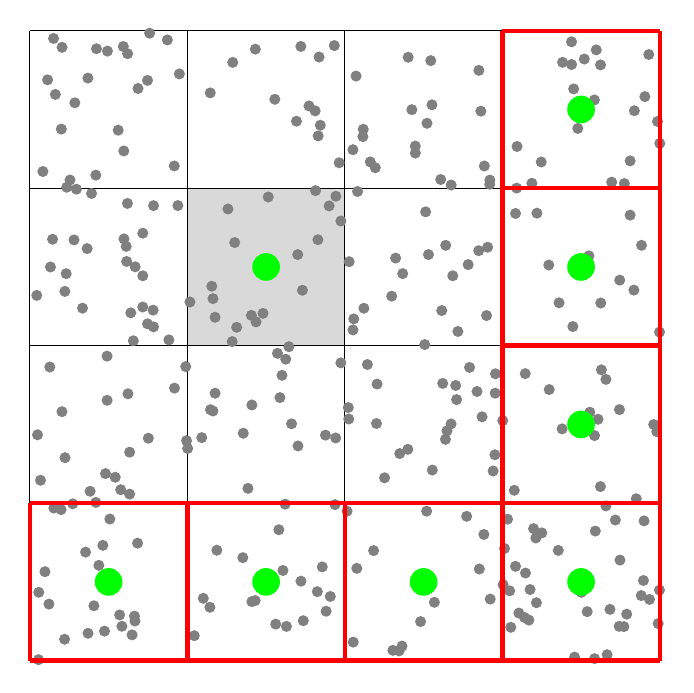
\begin{tikzpicture}
        \pgfmathsetseed{42}

        \fill[gray!30] (2,4) rectangle (4,6);

        \draw[step=2            ] (0,0) grid (8,8);

        \foreach \x in {1,...,180} {
          \fill[gray] (rnd*6, rnd*6+2) circle (2pt);
        }
        \foreach \x in {1,...,80} {
          \fill[gray] (rnd*8, rnd*2) circle (2pt);
        }
        \foreach \x in {1,...,60} {
          \fill[gray] (rnd*2+6, rnd*8) circle (2pt);
        }

        \fill[color=green] (3,5) circle (5pt);
        \foreach \x in {1,3,5,7} {
          \fill[color=green] (\x,1) circle (5pt);
        }
        \foreach \y in {3,5,7} {
          \fill[color=green] (7,\y) circle (5pt);
        }

        \draw[step=2, ultra thick, red] (0,0) grid (8,2);
        \draw[step=2, ultra thick, red] (6,0) grid (8,8);
      \end{tikzpicture}
      }
    }
    \caption{Step 4 of \gls{fmm}}
    \label{fig:step4}
  \end{figure}


  However, there is still a number of boxes that are well-separated from the green box but are not well-separated from its parent.
  And these boxes contribute to the incoming expansion of the blue box labeled as $\tau$ in \cref{fig:step4.1}, but they did not contribute to the incoming expansion for the parent, so we need to explicitly add these.
  The incoming expansion $u^\tau$ is then constructed via the incoming-from-incoming translation operator.
  The incoming-from-incoming translation operator results from truncating the series to the first $P$ terms \cite{Martinsson2015}:
  \begin{equation}
    \hat{\vct u}_{k}^{\sigma}=\sum_{j=k}^{\infty} \hat{\vct u}_{j}^{\tau}\mat{j \\ k} \left(\boldsymbol{c}_{\sigma}-\boldsymbol{c}_{\tau}\right)^{j-k}
  \end{equation}

  We continue this way and compute the incoming expansion for each box and we eventually hit the leaves.
  All that remains is then to expand the incoming expansion into potentials and adding the contributions from sources in the neighbor area via direct computations.

  \begin{figure}
    \centering
    \subfloat{
     \resizebox{4cm}{4cm}{%
      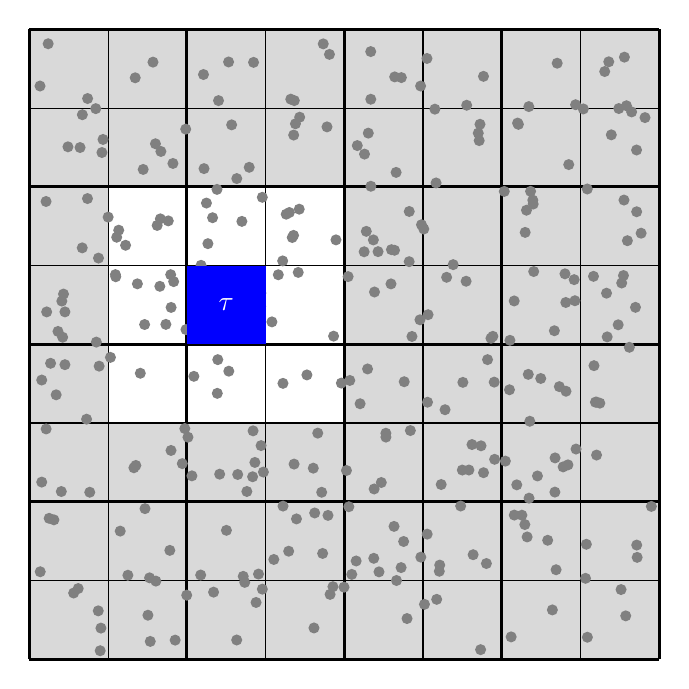
\begin{tikzpicture}
        \fill[gray!30] (0, 6) rectangle (8, 8);
        \fill[gray!30] (0, 0) rectangle (1, 6);
        \fill[gray!30] (0, 0) rectangle (8, 3);
        \fill[gray!30] (4, 0) rectangle (8, 8);

        \draw[step=1            ] (0,0) grid (8,8);
        \draw[step=2, very thick] (0,0) grid (8,8);

        \foreach \x in {1,...,320} {
          \fill[gray] (rnd*7.8+0.1, rnd*7.8+0.1) circle (2pt);
        }

        \fill[blue] (2,4) rectangle (3,5);
        \node[white] at (2.5, 4.5) {$\tau$};
      \end{tikzpicture}
      }
    }\hspace{4em}\subfloat{
     \resizebox{4cm}{4cm}{%
      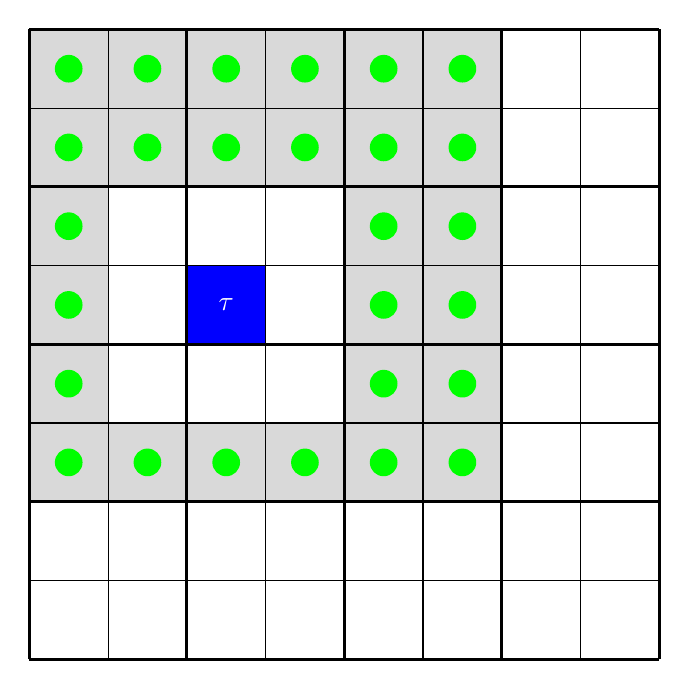
\begin{tikzpicture}
        \fill[blue] (2,4) rectangle (3,5);
        \node[white] at (2.5, 4.5) {$\tau$};

        \fill[gray!30] (0, 6) rectangle (6, 8);
        \fill[gray!30] (0, 2) rectangle (1, 6);
        \fill[gray!30] (0, 2) rectangle (6, 3);
        \fill[gray!30] (4, 2) rectangle (6, 8);

        \draw[step=1            ] (0,0) grid (8,8);
        \draw[step=2, very thick] (0,0) grid (8,8);

        \foreach \x in {0.5, 1.5, ..., 5.5}
        \foreach \y in {2.5, 6.5, 7.5} {
          \fill[color=green] (\x,\y) circle (5pt);
        }
        \foreach \x in {0.5, 4.5, 5.5}
        \foreach \y in {3.5, 4.5, 5.5} {
          \fill[color=green] (\x,\y) circle (5pt);
        }
      \end{tikzpicture}
      }
    }
     \caption{Step 4 of \gls{fmm}}
    \label{fig:step4.1}
  \end{figure}

  \item Compute: $\vct{u}\left(I_{\tau}\right)=\vct{T}_{\tau}^{\mathrm{tfi}}\hat{\vct{u}}^{\tau}+\vct{A}\left(I_{\tau}, I_{\tau}\right) \vct{q}\left(I_{\tau}\right)+\sum_{\sigma \in \mathcal{L}_{\tau}^{\mathrm{nei}}} \vct{A}\left(I_{\tau}, I_{\sigma}\right) \vct{q}\left(I_{\sigma}\right)$

  The blue marked box in \cref{fig:step5} is a leaf.
  We want to evaluate the potential inside the leaf.
  Everything is well-separated.
  Far-field contributions are evaluated by simply expanding the incoming expansion, which is done using the target-from-incoming translation operator.
  Then we need to add the near-field/neighbor interactions.
  These are not well-separated, and therefore, this is done via direct computation.

  \begin{figure}
    \centering
    \resizebox{4cm}{4cm}{%
    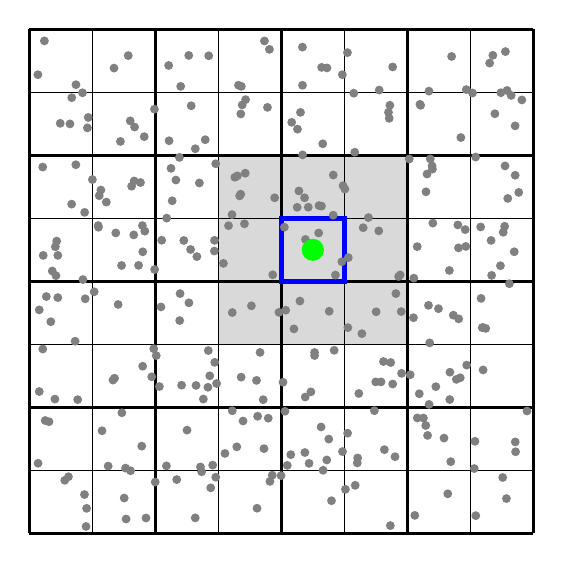
\begin{tikzpicture}[scale=0.8]
      \fill[gray!30] (3, 3) rectangle (6, 6);

      \draw[step=1            ] (0,0) grid (8,8);
      \draw[step=2, very thick] (0,0) grid (8,8);

      \draw[blue, ultra thick] (4, 4) rectangle (5, 5);

      \foreach \x in {1,...,320} {
        \fill[gray] (rnd*7.8+0.1, rnd*7.8+0.1) circle (2pt);
      }

      \fill[color=green] (4.5, 4.5) circle (5pt);
    \end{tikzpicture}}
    \caption{Step 5 of \gls{fmm}}
    \label{fig:step5}
  \end{figure}
\end{enumerate}

The steps 2 and 3 of the algorithms are also known as the upwards pass (we traverse the quad-tree from the leaves up), while steps 4 and 5 are known as the downwards pass (we start at the root and work our way down to the leaves).

\subsection{Error Analysis}

Due to the fact that all expansions have been reduced to $P$ terms, the potentials estimated by the \gls{fmm} are not precise.
In most cases, the global error is similar to the worst-case local truncation error \cite{articleErick}.
In other words, it scales as  $\alpha^P$ where  $\alpha = \frac{\sqrt{2}}{4-\sqrt{2}} \approx 0.5469$.
Therefore, we can see that to achieve a given tolerance $\epsilon$, then $P \approx \frac{\log (\epsilon)}{\log (\alpha)}$ \cite{Martinsson2015}.
Moreover, if we assume that each leaf holds $\mathcal{O}(P)$ sources, then increasing $P$ means that the asymptotic complexity of the 2D \gls{fmm} is $\mathcal{O}(P N)$.
As a result, the overall complexity scales as $\log (\frac 1 \epsilon) N$ as $\epsilon \rightarrow 0$ and $N \rightarrow \infty$ \cite{Martinsson2015}.
